\chapter{Custos e viabilidade}

  Esta seção apresenta os custos estimados inerentes à solução proposta neste trabalho.
  
   \section{Custos com mão de obra}
   
      Nesta seção são considerados os custos com os profissionais necessários para a execução do projeto.
      
      \subsection{Gerência}
		
	\begin{itemize}
	 
	  \item Gerente de Qualidade: 6500,00;
		  \subitem Total = 3 meses x 6500,00 = 19500,00.
	  \item Gerente de Projeto: 5000,00;
		  \subitem Total = 3 meses x 5000,00 = 15000,00.
	  \item Gerente de Custos: 10000,00;
		  \subitem Total = 3 meses x 10000,00 = 30000.00.
	  \item Gerente de Contrato (Recursos humanos): 5000,00;
		  \subitem Total = 3 meses x 5000,00 = 15000,00.
	  \item Gerente de Compras/Logística (Aquisição): 7000,00;
		  \subitem Total = 3 meses x 7000,00 = 21000,00.
	  \item Gerente de planejamento (Scopo): 4500,00;
		  \subitem Total = 3 meses x 4500,00 = 13500,00.
	  \item Gerente de inteligência de mercado/ Planejamento estratégico: 12000,00;
		  \subitem Total = 3 meses x 12000,00 = 36000,00.
	  \item Gerente de integração: 7000,00;
		  \subitem Total = 3 meses x 7000,00 = 21000,00.
	  \item Gerente/Coordenador de comunicação: 5000,00.
		  \subitem Total = 3 meses x 5000,00 = 15000,00.

	\end{itemize}

	\emph{\textbf{Total gerência}: R\$ 186.000,00.}
	
      \subsection{Analistas}
      
	\begin{itemize}

	  \item Recursos Humanos:
		\subitem  -Analista de Recursos Humanos: 3700,00; 2x 
		\subitem  Total = 2 x 3700,00  = 7400,00 x 3meses = 22200.00.
	  \item Custos:
		\subitem Analista de custos e Orçamento: 3700,00; 2x
		\subitem 	  Total = 2 x 3700,00 = 7400,00 x 3 meses = 22200,00.
	  \item Qualidade:
		  \subitem Analista de Controle de Qualidade: 4000,00; 2x
		  \subitem Total = 2 x 4000,00 = 8000,00 x 3 meses = 24000,00.
	  \item Aquisição:
		  \subitem Analista de Aquisição: 3600,00; 2x
		  \subitem Total = 2 x 3600,00 = 7200,00 x 3 meses = 21600,00.
	  \item Riscos:
		  \subitem Analista de Riscos:  5000,00; 2x
			  \subitem Total = 2 x 5000,00 = 10000,00 x 3 meses = 30000,00.
	  \item Tempo:
		  \subitem Analista de tempo (Planejamento): 6000,00; 2x
			 \subitem  Total = 2 x 6000,00 = 12000,00 x 3 meses = 36000,00.

	  \item Comunicação:
		  \subitem Analista de comunicação: 1600,00; 2x
			\subitem   Total = 2 x 1600,00 = 3200,00 x 3 meses = 9600,00.
	  \item Escopo:
		  \subitem Analista de escopo (Planejamento): 6000,00; 2x
			 \subitem  Total = 2 x 6000,00 = 12000,00 x 3 meses = 36000,00.
	  \item Integração:
		  \subitem Analista de Projeto: 4200,00; 2x
			  \subitem Total = 2 x 4200,00 = 8400,00 x 3 meses = 25200,00.
	\end{itemize}

	\emph{\textbf{Total analista}: R\$ 226.000,00.}
	
      \subsection{Desenvolvimento do \textit{Software}}
      
	O desenvolvimento será orientado no processo de desenvolvimento de
	Software ágil, assim sendo o mesmo utilizará como metodologia de gerência de
	projeto o Scrum. Deste modo, ocorrerá a divisão do escopo do projeto em
	Sprints, assim será utilizado como base o escopo do projeto definido no
	Documento de visão, distribuído em Sprints, e consequentemente em uma
	análise de custo por hora de desenvolvimento, referente aos funcionários
	estabelecidos no projeto.
	
	Segundo Kem Schwaber e Jeff Sutherland (2013), desenvolvedores do
	guia do Scrum, estabelecem como o tempo recomendado de uma Sprint, de
	aproximadamente duas semanas.
	
	O \textit{backlog} referente as Sprints será composto primariamente dos
	Requisitos Funcionais do sistema, sendo refinado posteriormente em histórias
	de usuário na fase de implementação dos mesmos.
	
	Como descrito no Documento de Visão (anexo \ref{doc_visao}) o sistema foi dividido em três
	subsistemas:
	
	\begin{enumerate}
	 \item Monitoramento mecânico e lógico das turbinas eólicas.
	 \item Monitoramento da qualidade da água
	 \item Monitoramento do reservatório de distribuição.
	\end{enumerate}
	
	Devido a dependência do desenvolvimento dos subsistemas, estes
	devem ser desenvolvidos de modo sequencial, uma vez que o subsistema 2,
	necessita de dados referentes ao sistema 1, e o subsistema 3 necessita de
	dados referentes aos subsistemas 2 e 1.
	
	\begin{table}[h]
	  \centering
	  \begin{tabular}{|c|c|}

	  \hline
	  \textit{\textbf{Sprint}} & \textbf{Requisitos Funcionais}\\
	  \hline
	    01 & RF01; RF02; RF03\\
	    \hline
	    02 & RF04; RF5; RF06\\
	    \hline
	    03 & RF07; RF08; RF09\\
	    \hline
	    04 & RF10; RF11; RF12\\
	    \hline
	    05 & RF13; RF14; RF15; RF16\\
	    \hline
	    06 & RF17; RF18; RF19\\
	    \hline
	    07 & RF20; RF21; RF22\\
	    \hline
	    08 & RF23; RF24; RF25\\
	    \hline
	    09 & RF26; RF27; RF28; RF29\\
	    \hline
	    10 & RF30; RF31; RF32; RF33; RF34;\\
	    \hline
	  \end{tabular}
	  \caption[Backlog das Sprints]{Backlog das Sprints.}
	\end{table}
	
	Com base no \textit{backlog} das \textit{sprints} o desenrolamento do Sistema de
	monitoramento do processo de captação e distribuição da agua, será realizado
	em cinco meses.
	
	Serão 9 envolvidos no desenvolvimento do projeto, sendo divididos em
	três principais áreas: gerência, analista de sistemas e desenvolvimento do
	software. Considerando o tempo estimado do projeto de 20 semanas, totalizando 
	600 horas, temos os seguintes custos \footnotemark:
	
	\begin{itemize}
	  \item 1 gerente de projeto (R\$94,70/hora);
	    \subitem Custo do Gerente: 94,70 x 600 = \textbf{R\$ 58.820,00}.
	  \item 3 analistas de sistema (R\$82,00/hora);
	    \subitem Custo dos analistas: 3 x 82,00 x 600 = \textbf{R\$ 147.600,00}.
	  \item 5 desenvolvedores (R\$60,00/hora).
	    \subitem Custo dos desenvolvedores: 5 x 60,00 x 600 = \textbf{R\$ 180.000,00}.
	\end{itemize}
	\footnotetext{Fonte dos dados salariais: <http://info.abril.com.br/noticias/carreira/fotonoticias/veja-a-media-salarial-dos-profissionais-de-ti-para-2015-1.shtml>}
	
	\emph{\textbf{Total da mão de obra do \textit{software}}: R\$ 384.420,00.}
	
      \subsection{Instalação das turbinas}
      
	A pesquisa a seguir foi realizada com base no Custo Unitário Básico de Construção (CUB), que é um indicador de custos no setor de construção regido pela Lei Federal 4.591/64.
	
	\FloatBarrier
	\begin{figure}[!h]
	    \centering
	    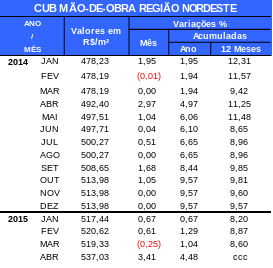
\includegraphics[scale = 1]{editaveis/figuras/cub_nordeste}
	    \caption[CUB na região nordeste]{CUB na região nordeste.}
	    \label{cub_nordeste}
	\end{figure}
	\FloatBarrier
	
	Com base na área total disponível para implantação do projeto, que é de 3,86 $km^2$, e levando em consideração o CUB Mão de obra da região nordeste no ano de 2015 mês Abril, chegamos aos seguintes resultados:
	
	$$ Area_{projeto} = 3,86 km^2 = 3860000 m^2$$
	
	$$ Preço_{m^2} * Area_{projeto} = 537,03 * 3860000 = R\$ 2.072.935.800,00.$$
	
	OBS: A responsabilidade de obra para instalar as turbinas, será de responsabilidade da prefeitura de Acari, assim como os gastos da mesma. Supondo uma parceria entre a empresa e a prefeitura.
	
    \section{Custos dos componentes}
      
      \subsection{Componentes mecânicos}
      
      \subsection{Componentes eletrônicos}
      
      \subsection{Componentes energéticos}
    
    \section{Custo total do projeto}
      
      Somando-se todos os custos apresentados, estima-se um valor de R\$
    
    \section{Estimativa de venda do produto}
    
      Analisando todos os gastos para a implantação do projeto, estimamos através da situação hipotética de uma provável venda da água,
      de 500ml e 20lt. O preço de uma garrafa de 500ml seria de três reais e o galão de 20lt de sete reais, contudo esse último haveria
      a necessidade da troca de galões. Se trabalharmos com a ideia de 26 dias no mês, vendendo no mínimo para a metade dos
      habitantes, a quantidade de 5.5lt de água por pessoa, obteríamos Trezentos e oitenta e seis mil e cem reais no final do
      mês, e chegando ao final do ano obteríamos Quatro milhões seiscentos e trinta e três mil e duzentos reais, levando em
      conta apenas as vendas de garrafas de 500ml.
      
      %       Tabela aqui
      
      Criando uma estimativa da quantidade de pessoas por famílias, analisando uma média de 4 pessoas por família, trabalharíamos
      para abastecer cerca de 225 famílias, pois a população do bairro é de 900 pessoas. Neste caso poderia ser vendido 1 galão 
      de 20lt e 4 garrafas de 500ml, fazendo para os mesmos 26 dias da hipótese anterior, vendendo para cerca de metade das
      famílias, as vendas daria um retorno menor, seria aproximadamente 112,5 famílias atendidas, com o galão vendido a sete 
      e a garrafinha com o mesmo valores, obteríamos aproximadamente, Um mil trezentos e cinquenta reais com a venda de 450
      garrafinhas e com a venda de 112,5 galões, cerca de Setecentos e oitenta e sete reais e cinquenta centavos. Ao dia daria,
      Dois mil cento e trinta e sete reais e cinquenta centavos. Após os 26 dias seria obtido Cinquenta e cinco mil quinhentos
      e setenta e cinco reais, pouco menos de 15\% do valor da situação anterior. Ao final do mês cinquenta e cinco mil 
      quinhentos e setenta e cinco reais e no final do ano seiscentos e sessenta e seis mil e novecentos reais.
      
      %       Tabela aqui
      
      Analisando a primeira situação de venda, com garrafinhas de 500ml apenas, o retorno do valor investido seria a partir do quinto mês, com o retorno de R\$1930500,00. Na segunda situação de venda, considerando os galões de 20lt, seria obtido o retorno apenas após dois anos e cinco meses, com o retorno de R\$1611675,00. Observando que seria preciso vender para no mínimo metade da população.
      
      Este projeto tem como grande enfoque, proporcionar à população, uma solução alternativa, devido à crise hídrica. Poderíamos até vender e com isso ter um grande lucro, pois todos os seres humanos precisam de água para o seu dia-a-dia, tornando viável economicamente. Contudo, a nossa ideia não pode ser estimada em custo, pois não a valor em poder ajudar pessoas que necessitam de um bem tão precioso como a água.
      
      Se fizermos uma comparação da água com a gasolina baseado no preço do estado do Rio grande do Norte, chegamos à conclusão que o litro de água é quase 100\% mais cara devido a gasolina em média custar Três reais e vinte e cinco centavos e a garrafinha de 500ml à Três reais. Se fossemos fazer o mesmo projeto voltado para a gasolina, um método alternativo de produzir a gasolina bateando-a, não iria ser tão viável, pelo fato ser muito complexo, requer um investimento muito grande e também porque o uso do combustível fóssil não traz benefícios ao meio ambiente e já existem outros tipos de combustíveis renováveis.  
      
   \section{Economia familiar}
   
      De acordo com a Organização das Nações Unidas, cada indivíduo precisa de 3,3 $m^3$ por mês, o que é cerca de 110
      litros de água por dia para atender as necessidades de consumo e higiene. No Brasil o consumo pode chegar a mais
      de 200 litros por dia.
      
      Dos cerca de 200 litros diários consumidos nos domicílios, segundo a Sabesp:
      \begin{itemize}
	\item 54 litros (27\%) - Cozinhar e beber.
	\item 50 litros (25\%) - Tomar banho e escovar os dentes.
	\item 66 litros (33\%) - Utilizados em descarga de banheiro.
	\item 24 litros (12\%) - Lavagem de roupa.
	\item 6 litros (3\%) - Outros (como lavagem de carro, por exemplo).
      \end{itemize}
      
      Na cidade de Acari há um rodízio onde a escala adotada utiliza o abastecimento por 24 horas e a interrupção por 48 horas,
      de forma a garantir um período mais prolongado de suprimento de água no manancial. Isso sucedeu-se pelo fato do Açude
      Gargalheiras está atuando hoje com menos de 6\% do seu volume total de armazenamento.
      
      Quando o fornecimento de água e coleta de esgotos sanitários forem usados para fins domésticos em economia de uso
      exclusivamente residencial a empresa do CAERN utiliza estes valores para tarifar a população.
      
      \FloatBarrier
      \begin{figure}[!h]
	  \centering
	  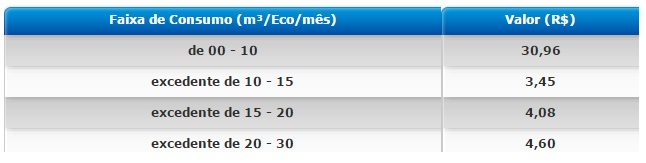
\includegraphics[scale = 0.9]{editaveis/figuras/custo_caern}
	  \caption[Tabela de tarifas da CAERN]{Tabela de tarifas da CAERN \footnotemark.}
	  \label{custo_caern}
      \end{figure}
      \footnotetext{Disponível em: <http://si.caern.com.br/gsan/exibirConsultarEstruturaTarifariaPortalCaernAction.do>}
      \FloatBarrier
      
      De acordo com a tabela mostrada acima, levantamos o valor que cada família pagaria se caso a quantidade de água fornecida fosse através da empresa CAERN. Na situação que criamos, cada família gastaria por mês Trinta reais e noventa e seis centavos, cada m3 cubico aproximadamente a Três reais e seis centavos pois cada família necessita de 22l de água por dia, ao mês, considerando ainda os 26 dias, teríamos 572l ou 0,572$m^3$. Valor este que se enquadra na taxa de consumo da primeira situação da tabela. Ao ano seria consumido cerca de 6,864$m^3$ e o gasto seria de Trezentos e setenta e um reais e cinquenta e dois centavos. 
      
      Analisando toda a estimativa feita e com os valores obtidos, vemos que geraria uma economia considerável para cada família.
      
      %       Tabela aqui
 